\chapter{Landauer's cost at body temperature}\label{ch:landauer}

\section{The cost of one bit}

At $\Tb=310.15$~K,
\begin{equation}
  e_{\mathrm{bit}}=\kB\Tb\ln2=(1.380649\times10^{-23})(310.15)(0.693147)
  =2.968\times10^{-21}\ \mathrm{J},
  \label{eq:ebit}
\end{equation}
or $1.787$~kJ per mole of bits. \calc{} This is the least free energy that must be dissipated to
make one irreversible binary commitment at body temperature. It is not the cost the cell actually
pays; it is the floor under whatever mechanism the cell uses.

\section{The Mahaffey number}

The cell's currency for irreversible work is ATP. Under cytosolic conditions the free energy of
hydrolysis is about $\dGATP\approx54$~kJ\,mol$^{-1}$, larger than the standard value of
30.5~kJ\,mol$^{-1}$ because the cell holds ATP far from equilibrium with ADP and
phosphate~\cite{Nelson2017}. The ratio of that drive to the thermal quantum is
\begin{equation}
  M=\frac{\dGATP}{R\Tb}=\frac{54\,000}{8.314462618\times310.15}=20.94 .
  \label{eq:M}
\end{equation}
\calc

\begin{definition}[Mahaffey number]
For any system that drives irreversible events with energy $\Edrive$ per event against a thermal
environment at temperature $T$,
\[
  M=\frac{\Edrive}{\kB T}.
\]
It is dimensionless and fixed by the physics of the drive. For the cell $M=20.94$; for a CMOS gate
at 75~\textdegree C with $\Edrive=3.9\times10^{-19}$~J, $M=81$~\cite{MahaffeyQuantumBook}.
\end{definition}

Two points of usage matter. First, $M$ is a constant of the cell's chemistry, not a reading of a
person: every human cell at 37~\textdegree C has the same $M$. Second, $M$ is defined without a
factor of $\ln2$ (author's ruling, 19 September 2026). The number of Landauer bits that one ATP can
pay for is then a separate quantity,
\begin{equation}
  \frac{M}{\ln2}=\frac{\dGATP}{N_A\,\kB\Tb\ln2}=30.21 .
  \label{eq:bitsperATP}
\end{equation}
\calc{} Figure~\ref{fig:budget} sets the two side by side.

\begin{figure}[t]\centering
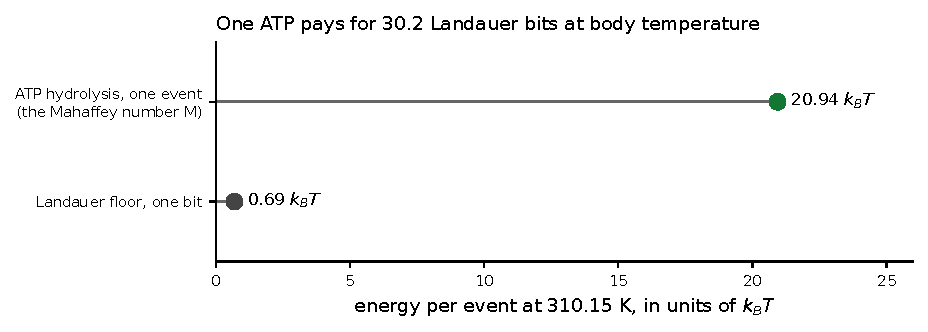
\includegraphics[width=0.85\textwidth]{figures/part4/fig_cell_budget.pdf}
\caption{Energy per event at body temperature in units of $\kB T$: the Landauer floor for one bit
($\ln2=0.69$) and one ATP hydrolysis under cytosolic conditions ($M=20.94$). \calc}
\label{fig:budget}
\end{figure}

\section{What a methyl mark costs the cell}

The methyl group on cytosine comes from $S$-adenosylmethionine (SAM). Methionine adenosyltransferase
builds SAM from methionine and ATP and releases all three phosphates, as pyrophosphate and
phosphate; pyrophosphate is then hydrolysed. The methyl transfer leaves $S$-adenosylhomocysteine,
which is hydrolysed and recycled to methionine through the folate and B$_{12}$ cycle, at further
cost. So each methyl mark costs the cell at least one ATP-equivalent, and in practice more.
\begin{equation}
  \frac{\text{chemical cost of one mark}}{\text{Landauer floor of one bit}}\gtrsim\frac{M}{\ln2}\approx30 .
  \label{eq:markmargin}
\end{equation}
\calc{} The cell pays at least thirty times the physical minimum for each bit it writes. That factor
is the \emph{cellular margin}: headroom between what the physics requires and what the chemistry
spends.

\section{The floor for one copy of the methylome}

At each S phase the cell copies its methylation pattern onto the new strands. DNMT1, recruited by
UHRF1 to hemimethylated CpGs at the replication fork, restores the methyl group opposite each
methylated parental CpG~\cite{Bostick2007,Sharif2007}. A human haploid genome carries about
28~million CpGs (hg38), of which roughly 70~\% are methylated in a typical somatic cell, so about
$19.6\times10^6$ marks are rewritten per new strand. That is the origin of the number used in the
source papers. The Landauer floor for that rewrite is
\begin{equation}
  E_{\mathrm{floor}}=N\,\kB\Tb\ln2=19.6\times10^6\times2.968\times10^{-21}
  =5.82\times10^{-14}\ \mathrm{J},
  \label{eq:efloor}
\end{equation}
equal to $6.5\times10^5$ ATP. \calc{} Figure~\ref{fig:divfloor} shows the floor for other ways of
counting the sites.

\begin{figure}[t]\centering
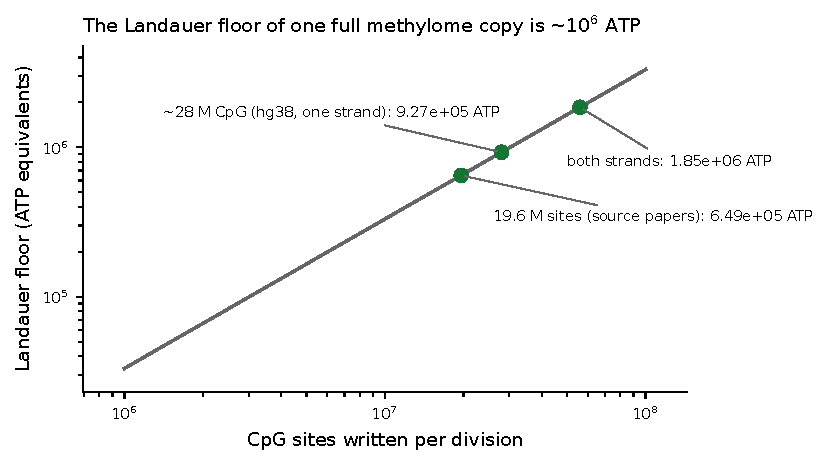
\includegraphics[width=0.72\textwidth]{figures/part4/fig_division_floor.pdf}
\caption{Landauer floor for one full rewrite of the methylation pattern, in ATP equivalents
($\dGATP=54$~kJ\,mol$^{-1}$), as a function of how many sites are counted. \calc}
\label{fig:divfloor}
\end{figure}

\begin{checkbox}
A mammalian cell turns over ATP at a rate of order $10^9$ per second~\cite{Milo2015}. Over a
24-hour cycle that is of order $10^{14}$ ATP. The chemical cost of one methylome copy, about
$2\times10^7$ ATP, is then a fraction of order $10^{-7}$ of the cell's energy budget, and the
Landauer floor is thirty times smaller again. \calc{} \emph{Energy is not what limits a cell's
methylation.} Whatever makes a cell lose or gain entropy on its identity loci, it is not that the
cell cannot afford the ATP. This is the first place where a naive reading of ``the cell cannot pay
its cost'' fails, and the book returns to it in Chapter~\ref{ch:floorbreach}.
\end{checkbox}

\section{Margin per write, and fidelity per write}

If total energy does not bind, what does? The answer the numbers point to is \emph{fidelity per
write}. A copying process that discriminates the right outcome from the wrong one by a free-energy
difference $\Delta\Delta G$ makes errors with probability of order $e^{-\Delta\Delta G/\kB T}$
(the equilibrium-discrimination limit; kinetic proofreading can do better at extra
cost~\cite{Hopfield1974}).

Hairpin-bisulfite measurements of maintenance methylation give per-site, per-division maintenance
efficiencies of about 0.95--0.98 and de novo rates of a few per cent~\cite{Genereux2005}. An error
rate of 2--5~\% corresponds to
\[
  \frac{\Delta\Delta G}{\kB T}=\ln\frac{1}{0.02\text{--}0.05}=3.0\text{--}3.9 .
\]
\calc{} The cell spends about $21\,\kB T$ per ATP and realises a discrimination of about $3$--$4\,\kB T$
per methylation decision. The large gap between the two is where the physics of methylation
lives.

\paragraph{The holding energy, measured on molecules.} The same quantity can be read directly on single DNA molecules.
On read-level whole-genome bisulfite data for 56 healthy human cell types~\cite{Loyfer2023}, the copy error $\varepsilon$
(an unmethylated CpG isolated between methylated neighbours, on molecules that are otherwise methylated) gives, through
$E_{\rm hold}=\kB T\ln[(1-\varepsilon)/\varepsilon]$, a holding energy of $3.41\pm0.12\,\kB T$ per site, range 3.13--3.72, in
every cell type (PROC-CHANNEL-01). \measured{} As a fraction of one ATP that is
\begin{equation}
  \phi=\frac{E_{\rm hold}}{M\,\kB T}=0.163\pm0.006 .
  \label{eq:phi}
\end{equation}
The value sits inside the range implied by the copying enzyme's own measured preference for hemimethylated over unmethylated
sites, 7--80-fold in vitro, which by Hopfield's relation is $\kB T\ln(\text{selectivity})=1.9$--$4.4\,\kB T$~\cite{Hopfield1974}.
That is a consistency check from independent biochemistry, not a confirmation. Chapter~\ref{ch:iama} turns
Eq.~\eqref{eq:phi} into the floor of the gauge. A cell's methylation pattern is not a static record: it is a steady state between a writing
process of finite fidelity and the cell's own divisions and demethylation, and its entropy on any
set of loci is set by that balance. Chapter~\ref{ch:surface} makes this precise.

\section{Where this stands: the information thermodynamics of methylation}\label{sec:sanchez}

That cytosine methylation obeys Landauer's bound is not new. Sanchez and Mackenzie~\cite{Sanchez2016} treated a change of methylation
state at a genomic region as an information-processing operation: with $p_i$ the methylation level at cytosine $i$, the information processed in a
region is the change of $\sum_i H(p_i)$, and the least energy dissipated to process it is that information times $\kB T\ln2$. They showed that the
distribution of this energy across regions, the background of methylation change set by thermal fluctuation, follows a Weibull distribution whose scale
recovers the persistence length of DNA (39--67~nm) from methylome data alone, and that regulatory signal can be separated from that background by
signal-detection theory. Their 2019 paper~\cite{Sanchez2019} turned this into a method (MethylIT): a Hellinger divergence of each sample from a
reference built from control individuals, a per-sample Weibull or gamma fit giving a critical value, and a classifier cutoff between
disease-induced and background change. \observed

Three things are taken from that work as established: $\kB T\ln2$ is the right physical anchor for methylation as a writing process; thermal
fluctuation produces a real statistical background in methylation level; and a measurement of methylation needs a reference from which departure is
measured. The approaches part at the third. In MethylIT the reference is the centre of a control group in the study at hand, re-established for every
cohort. Here it is fixed by the physics and by the healthy cell of the same kind, so that one specimen is read with no other specimen in the room
(Chapters~\ref{ch:meta} and~\ref{ch:iama}). Sanchez and Mackenzie use $\kB T$ as the scale of a background to be filtered; this book uses it as the
unit of measure. One filters; the other calibrates.

The two are complementary. Their background model is a principled way to ask which identity sites carry regulatory rather than thermal signal, a
question answered here by site selection, and it is the first extension to test. \prediction{} In the other direction, the calibration discipline of
Chapter~\ref{ch:instrument} applies to any absolute methylation measurement, including one built on divergences: a divergence from a control pool
inherits that pool's laboratory offset, which on arrays (0.066 in $\beta$ between two pipelines at the identity sites) is larger than the whole
Normal band. \measured{} Three differences limit the comparison: their data are sequencing read counts and the array results here are statements
about arrays; their signal is a site that moved, while a reading here is a cell against its reference; and their proposal of a binary methylation
``language'' is not used or evaluated. The author reached the question independently, from the thermodynamics of bound systems, and read their paper
after the first reference values had been frozen.

\section{Summary}
\begin{center}\small
\begin{tabular}{@{}lll@{}}\toprule
quantity & value & status \\\midrule
$\kB\Tb\ln2$ & $2.968\times10^{-21}$ J & \calc \\
$M=\dGATP/R\Tb$ & 20.94 & \calc \\
Landauer bits per ATP, $M/\ln2$ & 30.21 & \calc \\
floor for $19.6\times10^6$ marks & $5.82\times10^{-14}$ J $=6.5\times10^5$ ATP & \calc \\
chemical cost per mark / floor & $\gtrsim30$ & \calc \\
maintenance discrimination & 3--4 $\kB T$ & \calc{} from~\cite{Genereux2005} \\
holding energy on molecules, 56 cell types & $3.41\pm0.12\,\kB T$ & \measured \\
$\phi=E_{\rm hold}/M\kB T$ & $0.163\pm0.006$ & \measured \\\bottomrule
\end{tabular}
\end{center}
